%Pince et dynamixel
\subsection{Servomoteurs - Dynamixel AX12}
\subsubsection{Caractéristiques}
\begin{itemize}
    \item Un servomoteur est un système asservi capable de maintenir une opposition à un effort statique; 
    \item C’est donc une sorte de moteur qui est capable d’atteindre une vitesse et un angle déterminé;
    \item On transmet au servomoteur des ordres sous forme d'une modulation à largeur d’impulsion appelée PWM;
    \item On envoi une impulsion et c’est le temps de l’impulsion qui détermine l’angle à fournir par les servomoteurs;
    \item Pour comprendre son utilisation je vais rappeler certaines de ces caractéristiques.
\end{itemize}

\begin{figure}[!ht]
    \centering
    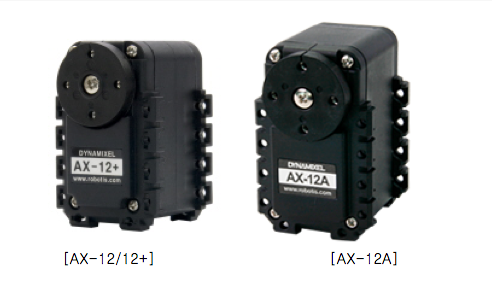
\includegraphics[scale=0.5]{AX.png}
    \caption{Dynamixels}
    \label{img:AX12}
\end{figure}

\paragraph{Caractéristiques du modèle AX12}
\begin{itemize}
    \item Poids : 54,6g;
    \item Dimension : 32mm * 50mm * 40mm;
    \item Angle autorisé : 0 à 300°;
    \item Résolution : 0.29°;
    \item Tension alimentation : 9 ~ 12V ;
    \item Type Protocole : Half duplex Asynchronous Serial Communication (8bit,1stop,No Parity);
    \item ID : de 254 identifiants possibles;
    \item Lecture possible : T°, tension, position.
\end{itemize}

\paragraph{Angle limite}

\begin{figure}[!ht]
    \centering
    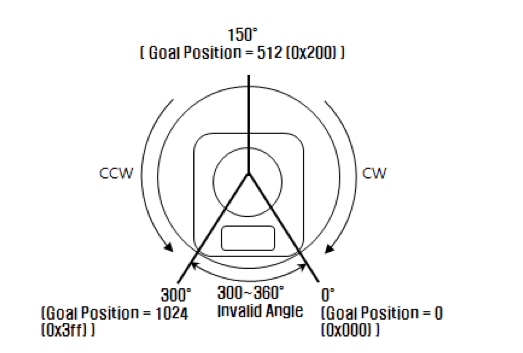
\includegraphics[scale=0.4]{angle.png} 
    \caption{Angle limite de la dynamixel}
    \label{img:angle_AX12}
\end{figure}

On peut aisément visualiser la position du 0° et la course possible du servomoteur sur la figure~\ref{img:angle_AX12}. Quand nous donnons une valeur d’angle nous la donnons de 0 à 1023 ce qui correspond à une valeur d’angle entre 0 et 300 °. Si je veux 150° je dois envoyer la valeur de 511,5 et mon servomoteur se positionnera en réalité à la position de notre 0 conventionnel. Si nous l’utilisons en « Wheel Mode » le servomoteur peut tourner sur 360° sans problème. 

\paragraph{Vitesse}
\subparagraph{Join Mode}
Nous envoyons une valeur entre 0 et 1023 où 1023 est la vitesse maximale du servomoteur. L’unité vaut 0,111rpm et la vitesse maximale est de 0,111*1023 = 113,553rpm (rotations par minute).
\subparagraph{Wheel mode}
En Wheel mode il faut connaitre la notion de CCW et CW qui correspondent respectivement à la rotation en sens anti horaire et la rotation en sens horaire. On peut utiliser des valeurs entre 0 et 2047. 

\subsection{Utilisation}
Pour utiliser les servomoteurs il faut d’abord intégrer la librairie "DynamixelSerial.h". Cette librairie contient toutes les fonctions déjà faites qui nous seront utiles pour utiliser
les servomoteurs. 

\noindent Notre objectif est de parcourir la liste et de se familiariser avec les différentes possibilités. 

\noindent Je vais tout d’abord décrire un certain nombre d’entre elles. 

\begin{enumerate}
     \item Dynamixel.begin(BaudRate, RxPin, TxPin, DataControl) \begin{itemize}
         \item On initialise la communication série avec l’arduino;
         \item RxPin est la pin de réception de données et TxPin pour la transmission de données.
     \end{itemize}
     
     \item Dynamixel.ping(ID)
     \begin{itemize}
        \item Connaître le statut du servomoteur.
     \end{itemize}
      
     \item Dynamixel.reset(ID)
     \begin{itemize}
        \item Rétablir les réglages par défaut du Dynamixel.
     \end{itemize}
      
     \item Dynamixel.setID(ID, new ID )
     \begin{itemize}
        \item Change l’ID du servomoteur.
     \end{itemize}
     
     \item Dynamixel.move(ID ,Position)
     \begin{itemize}
        \item Déplace la dynamixel jusqu’à la position correspondante, de 0 à 1023.
     \end{itemize}
     
     \item Dynamixel.movespeed(ID,Position,Speed)
     \begin{itemize}
        \item On précise en plus la vitesse voulue.
     \end{itemize}
     
     \item Dynamixel.moveRW(ID,Position)
     \begin{itemize}
        \item Enregistre l’instruction qui déplace le mécanisme jusqu’à une position correspondante.
     \end{itemize}
     
     \item Dynamixel.moveSpeedRW(ID,Position,Speed)
     \begin{itemize}
        \item Enregistre l’instruction.
     \end{itemize}
     
     \item Dynamixel.action()
     \begin{itemize}
        \item Exécute l’instruction sauvegardée dans le servo.
     \end{itemize}
     
     \item Dynamixel.setEndless(ID,Status)
     \begin{itemize}
        \item Active ou désactive la rotation en continue du servomoteur;
        \item Statut : ON/OFF.
     \end{itemize}
     
     \item Dynamixel.turn(ID,Side,Speed)
     \begin{itemize}
         \item ID - Identifiant Servomoteur;
         \item Sens de rotation RIGHT/LEFT;
         \item Speed : Vitesse de 0 à 1023.
     \end{itemize}
     
     \item Dynamixel.torqueStatus(ID,Status)
     \begin{itemize}
        \item Active ou désactive le mode couple du servomoteur.
     \end{itemize}
     
     \item Dynamixel.LEDStatus(ID,Status)
     \begin{itemize}
        \item Active ou désactive la LED.
     \end{itemize}
     
     \item Dynamixel.readPosition(ID)
     \begin{itemize}
        \item Renvoi  la valeur de la position.
     \end{itemize}
     
     \item Dynamixel.readSpeed(ID)
     \begin{itemize}
        \item Renvoi la vitesse en RPM.
     \end{itemize}
\end{enumerate}

\subsection{Pince}
Cette année notre robot devra effectuer certaines tâches nécessitant l’utilisation d’une pince. Nous avons tout d’abord cherché à savoir ce qui existait déjà dans le commerce. Mais nous avons très vite renoncé à cette idée en se basant sur 2 réflexions : 

\begin{itemize}
    \item Prix d’achat trop élevé;
    \item Utilisation des Dynamixel déjà étudiée lors du projet Eurobot or la plupart des pinces fonctionnent avec des servomoteurs d’un autre type. Il aurait fallu tout recommencer.
\end{itemize}

\paragraph{}
En partant sur cette réflexion nous nous sommes rapidement lancés dans la conception de notre propre pince qui serait imprimée grâce à l’imprimante 3D. Les objets à porter sont :

\begin{itemize}
\item Verres simples;
\item Plots en bois ;
\item Balles en polystyrène.
\end{itemize}

\paragraph{}
Il nous faudra donc une pince classique avec deux doigts qui se referment. Nous étions partis là-dessus lors de la conception mais j’ai pensé à réutiliser le système des pinces à cheveux qui se referment. En croisant les doigts comme la pince à cheveux on pourra mieux attraper les objets comme des balles de ping pong.

\begin{figure}[!ht]
    \centering
    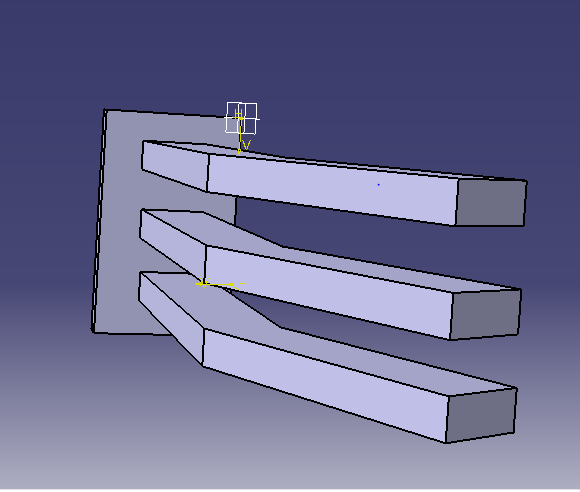
\includegraphics[scale=0.5]{pince2.png}
    \caption{Pince faite sur Catia, partie de gauche}
\end{figure}

\begin{figure}[!ht]
    \centering
    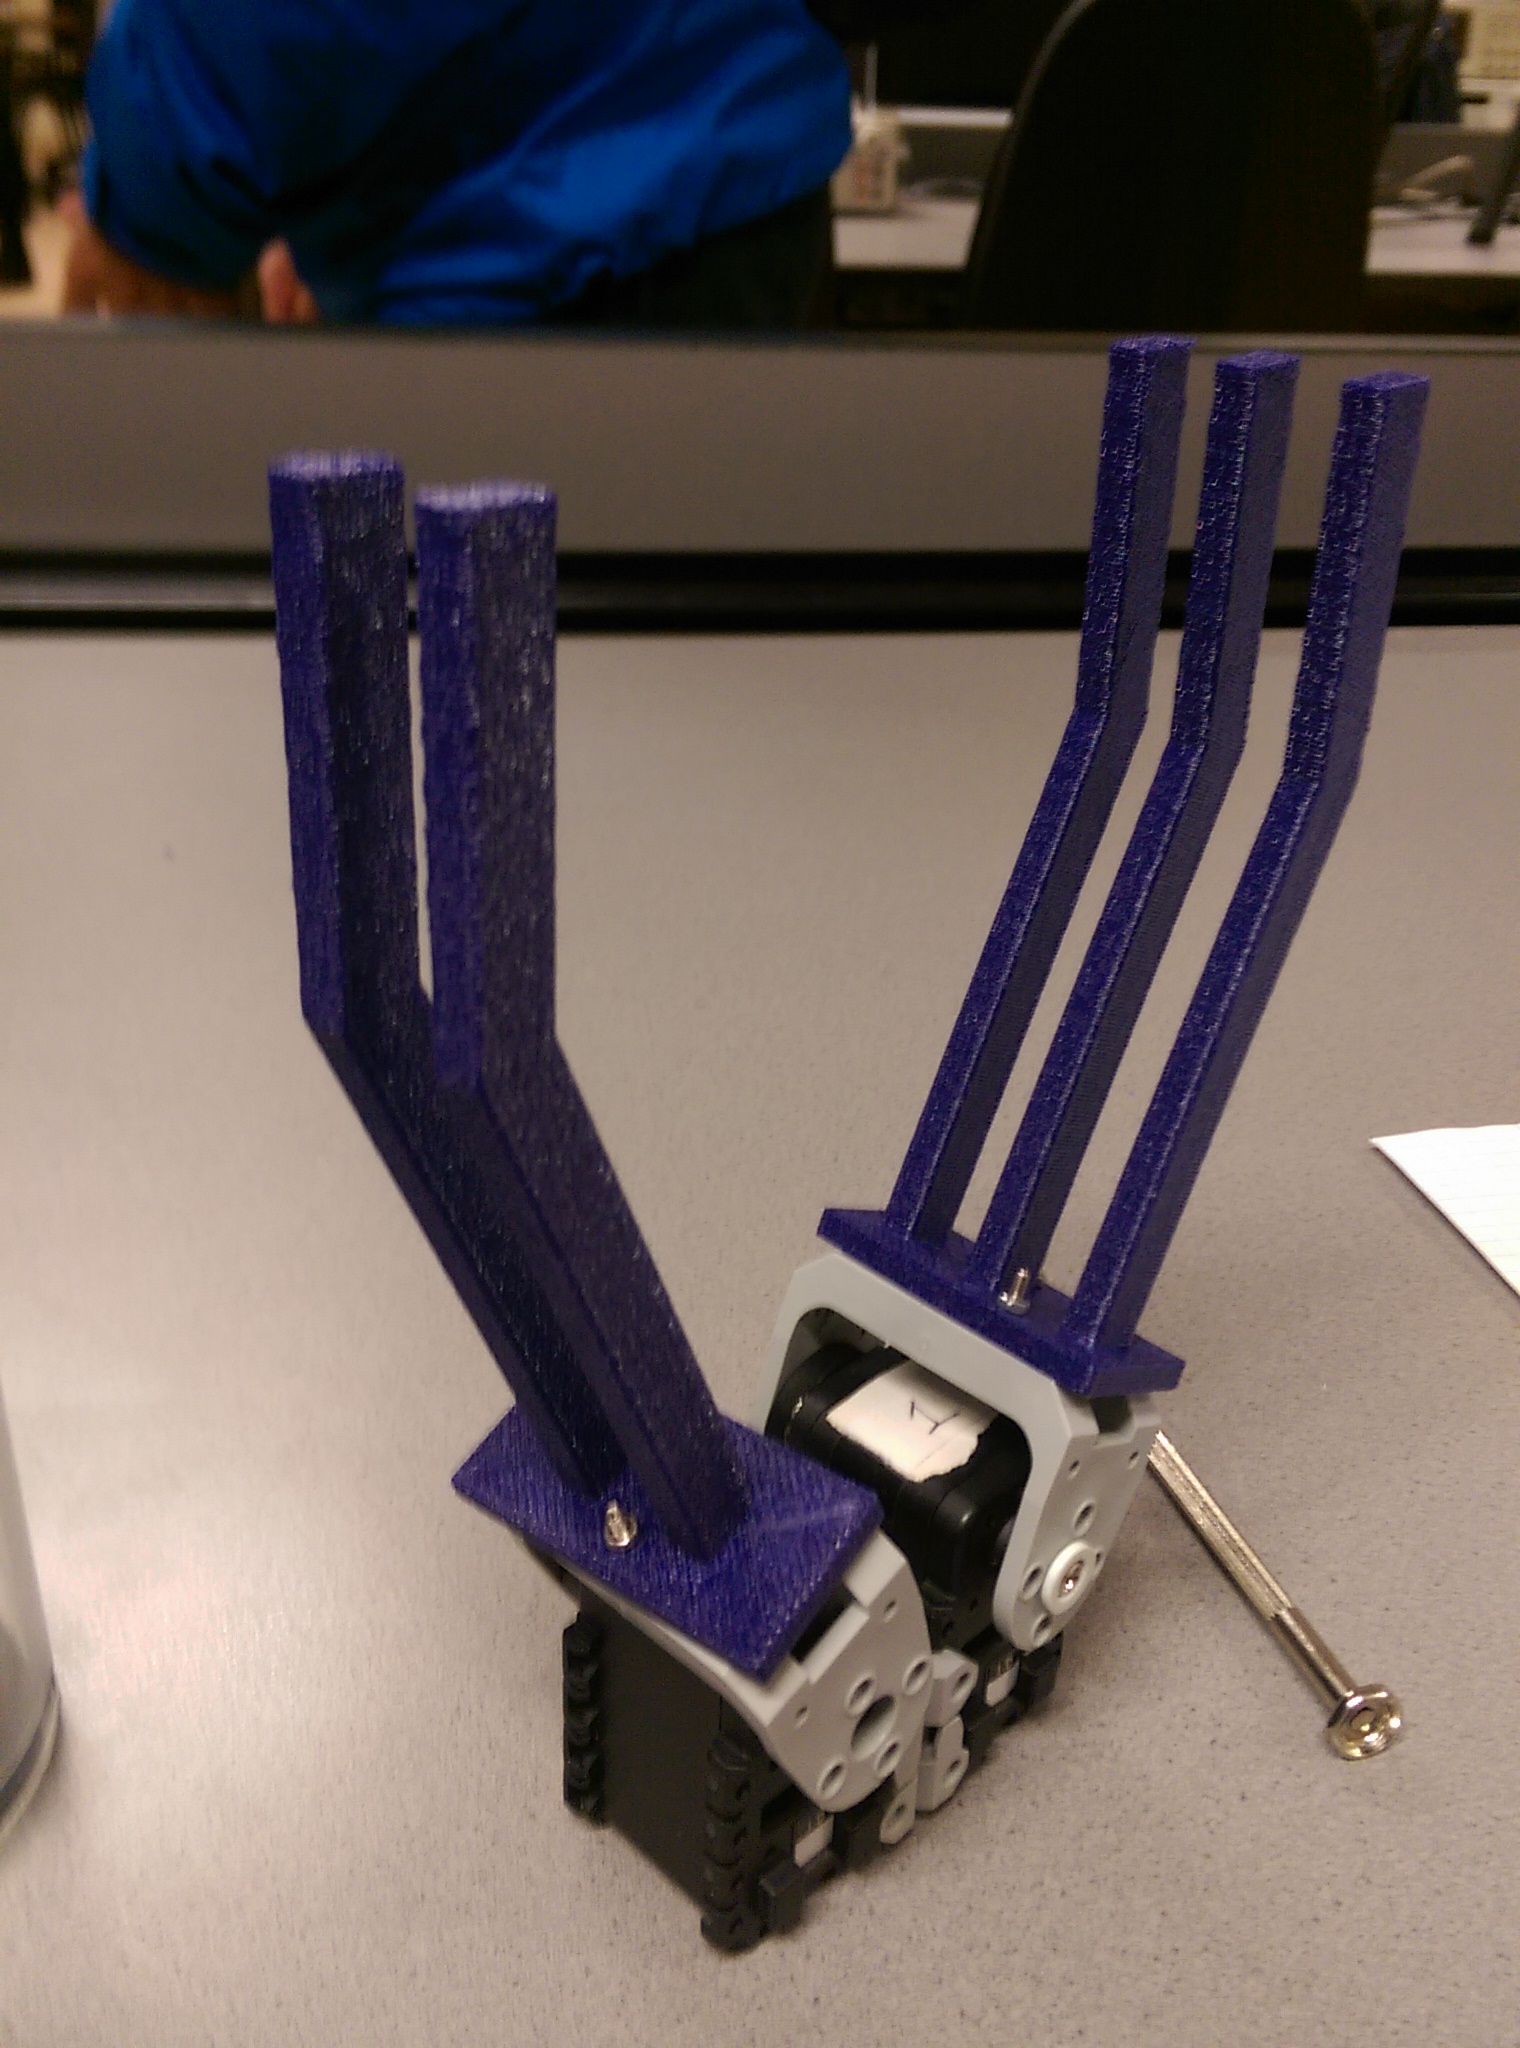
\includegraphics[width=10 cm]{pince1.jpg}
    \caption{Prototype de la pince (version légère}
    \label{fig:Pince1}
\end{figure}

\noindent Cette version qui est devenue la version finale a donc 3 doigts à droite et 2 doigts à gauches capables de se croiser (figure~\ref{fig:Pince1}). Les deux côtés sont chacun reliés à une Dynamixel qui sera contrôlée par une Arduino.

\noindent Cette pince sera elle même accrochée sur un rail qui lui permettra de faire des déplacements verticaux. La courroie sera guidée par une 3\up{ème} Dynamixel. On pourra ainsi faire monter, descendre, ouvrir et fermer selon un angle bien précis la pince grâce aux fonctions étudiées plus haut. 
Toute l'étude des couples et des objets à porter sera étudiée plus tard.